% 第 7 章
\section{从估计到推断：协方差、精度矩阵与条件独立}\label{sec:ggm}

第 \ref{sec:onedim} 章在一维世界里弄清了「相关 $\neq$ 因果」。本章把问题升格到联合层面：把 $(y, \x)$ 当作一个 $(d{+}1)$ 维随机向量，问\textbf{协方差矩阵与它的逆（精度矩阵）}如何编码 $y$ 与 $\X$ 之间的相关、条件独立与（在图假设下的）因果结构；再回答实践问题：$d$ 很大、$n$ 很小时如何估计（lasso、elastic net、CLIME、graphical lasso），以及如何把「点估计」升级为「推断」（debiased lasso）——即\textbf{from estimate to inference}。

\subsection{协方差与精度矩阵：相关的两种编码}\label{sec:cov-prec}

设 $(y, \x)$ 联合高斯，均值不妨为零，记
\[
  \bm{\Sigma} = \Cov\begin{pmatrix} y \\ \x \end{pmatrix} \succ \zero,
  \qquad
  \bm{\Theta} = \bm{\Sigma}^{-1} \ \text{(精度矩阵, precision matrix)}.
\]
两个矩阵编码两种不同的「相关」：

\begin{itemize}
  \item \textbf{协方差 $\Sigma_{ij} \neq 0$}：边际相关（marginal correlation）。它会\textit{传导}：即使 $y \perp x_j$ 在控制其余变量后成立（无直接联系），$x_j$ 仍可与 $y$ 边际相关——只要存在一条经其他变量的间接路径（第 \ref{sec:1d-causality} 节共同原因结构的多变量版本）。
  \item \textbf{精度矩阵元 $\Theta_{ij} = 0$}：\textbf{条件独立}。高斯情形有精确恒等式
  \begin{equation}\label{eq:ci-prec}
    \Theta_{ij} = 0
    \quad\Longleftrightarrow\quad
    i \perp j \mid \text{其余所有变量},
    \qquad
    \rho_{ij \cdot V \setminus \{i,j\}} = -\frac{\Theta_{ij}}{\sqrt{\Theta_{ii}\,\Theta_{jj}}} \ \text{(偏相关系数)} .
  \end{equation}
  即：\textit{偏相关为零 $\Leftrightarrow$ 在给定其他一切变量的条件下两者独立}。证明只需分块求逆（练习 \ref{ex:block-inv}）。
\end{itemize}

\eqref{eq:ci-prec} 是本章的枢纽：\textbf{精度矩阵的零模式是一张「条件独立图」的邻接矩阵}——高斯图模型（Gaussian graphical model）\cite{lauritzen1996}。相关沿图\textit{流动}（间接路径也产生相关），条件独立只在\textit{无边}时成立；这张图就是 Wright 路径图（第 \ref{sec:1d-causality} 节）的高斯化身。

\subsection{回归系数是精度矩阵的元素}\label{sec:beta-theta}

现在把线性回归接上这张图。对联合高斯做分块：$\bm{\Theta} = \begin{pmatrix} \Theta_{yy} & \bm{\Theta}_{yX} \\ \bm{\Theta}_{Xy} & \bm{\Theta}_{XX} \end{pmatrix}$（标量 $\Theta_{yy} > 0$，$\bm{\Theta}_{Xy} \in \R^d$）。由分块求逆（练习 \ref{ex:block-inv}），给定 $\X$ 时 $y$ 的条件分布为
\begin{equation}\label{eq:conditional}
  y \mid \X \sim \mathcal{N}\Big( -\tfrac{1}{\Theta_{yy}}\, \bm{\Theta}_{yX}^\top \x,\ \tfrac{1}{\Theta_{yy}} \Big).
\end{equation}
与回归模型 $y = \x^\top \bbeta + \varepsilon$ 对照，得到一组应当刻在石头上的恒等式：
\begin{equation}\label{eq:beta-theta}
  \boxed{\;\bbeta = -\frac{\bm{\Theta}_{Xy}}{\Theta_{yy}}, \qquad \Var(\varepsilon) = \frac{1}{\Theta_{yy}}\;}
\end{equation}

\begin{keybox}[回归 = 探查图结构]
\eqref{eq:beta-theta} 说：\textbf{回归系数（及其符号、显著性）是精度矩阵元素的比值}。特别地，
\[
  \beta_j = 0
  \quad\Longleftrightarrow\quad
  \Theta_{Xy,j} = 0
  \quad\Longleftrightarrow\quad
  y \perp x_j \mid \x_{-j}
  \ \text{（在控制其余特征后，$y$ 与 $x_j$ 条件独立）}.
\]
\end{keybox}

这句话把一个统计问题翻译成两个问题：
\begin{enumerate}[label=(\arabic*)]
  \item \textbf{相关}（第 \ref{sec:onedim} 章）：$y$ 与 $x_j$ 是否边际相关？——看 $\Sigma$，一个 $t$ 检验的事；
  \item \textbf{条件独立}：控制其余变量后，$y$ 与 $x_j$ 是否仍有「直接」联系？——看 $\Theta$ 的零模式，即\textbf{偏相关}是否为零。
\end{enumerate}
两者的差距正是「$x_j$ 与 $y$ 的相关完全由第三个变量解释」这类现象（混杂、中介）的矩阵语言。注意 $\beta_j = 0$ 给出的是\textbf{图论意义上的「无直接边」}，而不是因果断言——除非图本身已被外部知识（第 \ref{sec:1d-causality} 节）或下文的条件独立检验约束到可识别。

\subsection{条件独立检验与因果：从相关到图}\label{sec:ci-causal}

\eqref{eq:ci-prec} 提供了\textbf{可检验的约束}：高斯图上每条缺失的边都对应一个「偏相关为零」的统计假设
\begin{equation}\label{eq:ci-test}
  H_0^{(ij)}:\ \rho_{ij\cdot V\setminus\{i,j\}} = 0
  \quad(\Longleftrightarrow\ \Theta_{ij} = 0),
\end{equation}
可用 Fisher 的 $z$ 变换在小维情形直接检验；在高维情形，逐个检验不再可行，但约束的逻辑不变。PC 算法（Spirtes, Glymour \& Scheines）展示了这套约束如何变成因果发现\cite{spirtes2000}：

\begin{enumerate}[label=(\alph*)]
  \item \textbf{删边}：对每对变量搜索条件集 $S$，一旦检验出 $i \perp j \mid S$ 就在 $i,j$ 间删去无向边——共同原因与间接路径在这条检验现形（这正是 Reichenbach 原理 \cite{reichenbach1956} 的可操作版本）；
  \item \textbf{定向}：对 $i - k - j$ 且 $i, j$ 不相邻的结构（v-结构），在 Markov + faithfulness 假设下可定向 $i \to k \leftarrow j$——\textbf{数据本身对一部分箭头给出了方向}；
  \item \textbf{传播}：Meek 规则把方向沿图继续传播。
\end{enumerate}

与第 \ref{sec:1d-causality} 节呼应：相关系数本身永不给方向，但\textbf{一组条件独立检验}能在「图 faithful 于分布」的额外假设下恢复出部分 DAG；因果结论的合法性仍然来自假设清单，而不是来自数据本身——只是现在假设可以被逐一检验、逐一反驳。

\subsection{稀疏性：为什么「大多数系数是零」是可计算的假设}\label{sec:sparsity}

前两节给出了图模型的语言：$d$ 个变量之间至多有 $\binom{d}{2}$ 条边、$d^2$ 个精度矩阵元素要估计。当 $d > n$ 时这是不可能完成的任务——除非我们愿意相信一件很具体的事：\textbf{真实的图是稀疏的}，大多数 $\Theta_{ij} = 0$。本节解释为什么这个假设不仅合理，而且是「可计算的」。

\textbf{稀疏性是可证伪的假设，不是祈祷。}「大多数系数为零」意味着图有 $s \ll d^2$ 条边；若真实边数 $s$ 满足 $s \log d \ll n$，则有一类方法（下一节）能以高概率\textbf{恰好}恢复图的结构。反过来，若数据真是稠密的，稀疏方法的失败会以「交叉验证选不出稳定结构」的形式诚实地暴露——这与第 \ref{sec:1d-causality} 章「先拟合、审计假设」的精神一致：稀疏假设可以且应当被审计。

\textbf{稀疏性从何而来？}三个独立的来源。(1) \textbf{科学的}：基因调控网络中每个基因只被少数转录因子调控，社交网络每人只有若干紧密联系人——「每行非零元有界」是许多领域的先验知识，对应数学上的 $s = O(d)$ 条边。(2) \textbf{统计的}：在适当设计下，稀疏模型的有效自由度 $\ll d$（见下），样本复杂度由\textbf{非零元个数}而非维数决定——这正是「高维统计」一词的本义：$d$ 可以大于 $n$，只要真实参数的支撑集小于 $n$。(3) \textbf{计算的}：稀疏性把一个 $d^2$ 维的连续优化问题变成「找哪些坐标非零 + 估它们的值」，而后者有明确的算法与误差界。

\textbf{稀疏性的三个面孔，一句话一个。}
\begin{enumerate}[label=(\arabic*)]
  \item \textbf{组合面孔}：模型选择——在 $2^d$ 个子集中找正确的一个。NP-hard 的一般问题在稀疏假设下可解（$s$ 小使搜索空间塌缩）。
  \item \textbf{几何面孔}：$\ell_0$ 球 $\{\bbeta : \norm{\bbeta}_0 \le s\}$ 非凸，$\ell_1$ 是它的\textbf{凸松弛}（严格的包络关系是 $\norm{\bbeta}_1 \le \sqrt{s}\,\norm{\bbeta}_2$；「凸包恰为 $\ell_1$ 球」只在 $s = 1$ 时成立）：松弛后的优化问题重新变凸，而松弛的代价（恢复条件）可用不相干性与限制特征值（restricted eigenvalue）定量刻画。
  \item \textbf{统计面孔}：有效自由度。lasso 拟合 $\X\widehat{\bbeta}$ 的自由度 $\widehat{df} = \E[\text{非零系数个数}]$——\textbf{稀疏模型的复杂度由它实际用到的变量数来计}，而不是由 $d$。这解释了为什么稀疏估计的方差可以远小于 $O(d/n)$。
\end{enumerate}

\textbf{一个诚实的提醒}：稀疏性是\textbf{关于世界的假设}，不是数学技巧。若真实信号是稠密但衰减的（如 $\beta_j \propto 1/j$），强稀疏方法会系统性漏掉弱信号——此时 ridge（稠密收缩）可能比 lasso 更诚实。选 lasso 还是 ridge，是在选你相信哪种世界；第 \ref{sec:hd-break} 节的偏差--方差语言给出了这个选择的定量权衡。

带着这三张面孔，下一节进入估计的具体方法：lasso、elastic net、graphical lasso 与 CLIME——四个方法，都是在用不同的优化形式把「稀疏」这枚假设钉进估计量里。

\subsection{估计：$d$ 大 $n$ 小时的四种正则化}\label{sec:ggm-estimate}

样本协方差 $\bm{S} = \frac{1}{n}\X^\top\X$（中心化后）在 $d > n$ 时奇异，$\bm{S}^{-1}$ 不存在——\textbf{没有正则化就没有精度矩阵}。四种思路，一个目标（稀疏 $\bm{\Theta}$）：

前两种直接作用于回归系数。lasso（Tibshirani, 1996）解
\begin{equation}\label{eq:lasso}
  \min_{\bbeta} \ \frac{1}{2n} \norm{\y - \X \bbeta}^2 + \lambda \norm{\bbeta}_1 ,
  \qquad
  \norm{\bbeta}_1 = \sum_{j=1}^d |\beta_j| ,
\end{equation}
$\ell_1$ 惩罚的几何（约束集的尖角）把部分坐标\textbf{恰好}压成 $0$，给出稀疏解。elastic net（Zou \& Hastie, 2005）把 $\ell_1$ 与 $\ell_2$ 组合：
\begin{equation}\label{eq:enet}
  \min_{\bbeta} \ \frac{1}{2n} \norm{\y - \X \bbeta}^2 + \lambda \Big( \alpha \norm{\bbeta}_1 + \tfrac{1-\alpha}{2} \norm{\bbeta}^2 \Big),
\end{equation}
$\ell_2$ 成分让\textbf{高度相关的一整组变量一起进模型}（lasso 在相关组内随机挑一个的毛病由此修复），适合基因表达等组内强相关的数据。后两种把惩罚搬到矩阵层：

\begin{itemize}
  \item \textbf{lasso}的节点回归用法（Meinshausen \& Bühlmann, 2006）：把每个变量对其余变量解一次 \eqref{eq:lasso}，谁的系数非零就在图上连谁——第 \ref{sec:beta-theta} 节说了这等价于从精度矩阵逐列恢复\cite{tibshirani1996,meinshausen2006}。
  \item \textbf{graphical lasso}（Friedman, Hastie \& Tibshirani, 2008）：直接惩罚精度矩阵的似然，
  \[
    \min_{\bm{\Theta} \succ \zero} \ \trace(\bm{S}\bm{\Theta}) - \log\det \bm{\Theta} + \lambda \norm{\bm{\Theta}}_1 ,
  \]
  一次估计全图；其最优性条件 $\bm{S} - \bm{\Theta}^{-1} + \lambda \bm{\Gamma} = \zero$（$\bm{\Gamma}$ 为次梯度）把估计与条件独立检验直接挂钩\cite{friedman2008}。
  \item \textbf{CLIME}（Cai, Liu \& Luo, 2011）：不碰似然，直接解
  \[
    \min_{\bm{\Theta}} \ \norm{\bm{\Theta}}_1 \quad \text{s.t.} \quad \norm{ \bm{S}\bm{\Theta} - \bm{I} }_{\max} \le \lambda ,
  \]
  即「找一个稀疏的、近似是 $\bm{S}$ 之逆的矩阵」。它是\textbf{线性规划}（逐列可解），无需 $\bm{\Theta} \succ \zero$ 的约束与 $\log\det$ 的计算，在更弱的假设下给出谱范数收敛率，且天然适配「$\bm{\Sigma}$ 不必稀疏、只有 $\bm{\Theta}$ 稀疏」的场景\cite{cai2011}。
\end{itemize}

四者的共性是偏差--方差交易（第 \ref{sec:hd-break} 节）在矩阵层的重演：$\lambda$ 把大量 $\Theta_{ij}$ 压成 $0$，用一点有偏换取协方差求逆的方差可控。图 \ref{fig:ch6-lassopath} 画出了 \eqref{eq:lasso} 的解随 $\lambda$ 变化的正则化路径。

\begin{figure}[htbp]
  \centering
  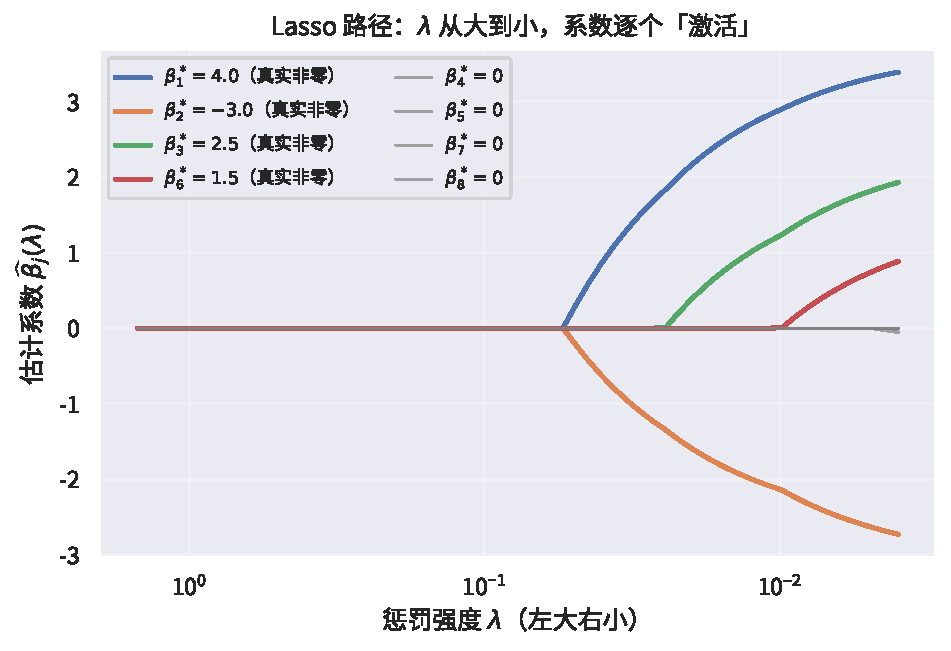
\includegraphics[width=0.85\linewidth]{figures/ch6_lassopath.pdf}
  \caption{Lasso 正则化路径（模拟数据，真实系数 $4,-3,2.5,0,0,1.5,0,0$）：$\lambda$ 从大到小（横轴左大右小），四个真实非零系数（彩线）依次从 $0$ 被「激活」，真实为零的系数（灰线）始终被压在 $0$ 附近——稀疏性不是假设出来的，是 $\ell_1$ 惩罚的几何（菱形约束角）自动选择的。}
  \label{fig:ch6-lassopath}
\end{figure}

\subsection{推断：debiased lasso 与条件独立的检验}\label{sec:debiased}

估计给出 $\hat\beta_j$ 之后，\textbf{点估计不能直接变成 $p$ 值}：lasso 的收缩使 $\hat\beta_j$ 有偏，其极限分布不是高斯。出路是\textbf{去偏}（debiasing / desparsifying）。思想一句话：\textit{把被惩罚偷走的项加回来}。取精度矩阵的 nodewise 估计 $\widehat{\bm{\Theta}}$（例如对 $\bm{S}$ 的每个节点做 lasso 回归、或直接用 CLIME），定义
\begin{equation}\label{eq:debiased}
  \widetilde{\bbeta} = \widehat{\bbeta}_{\mathrm{lasso}} + \tfrac{1}{n}\, \widehat{\bm{\Theta}}\, \X^\top \big( \y - \X \widehat{\bbeta}_{\mathrm{lasso}} \big).
\end{equation}
代数上看（练习 \ref{ex:debiased}）：$\widetilde{\bbeta} - \bbeta = \frac{1}{n}\widehat{\bm{\Theta}}\X^\top \bm{\varepsilon} + (\bm{I} - \widehat{\bm{\Theta}}\bm{S})(\bbeta - \widehat{\bbeta}_{\mathrm{lasso}})$——第一项是噪声（渐近正态），第二项是残余偏差（在稀疏性条件下 $o_p(n^{-1/2})$）。于是（Zhang \& Zhang, 2014; van de Geer et al., 2014）
\begin{equation}\label{eq:asym-norm}
  \sqrt{n}\, \big( \widetilde{\beta}_j - \beta_j \big) \ \xrightarrow{d}\ \mathcal{N}\Big( 0,\ \sigma^2 \big( \bm{\Theta}\, \bm{\Sigma}\, \bm{\Theta} \big)_{jj} \Big),
  \qquad
  \text{置信区间：}\ \widetilde{\beta}_j \pm z_{1-\alpha/2}\, \frac{\hat\sigma}{\sqrt{n}} \sqrt{ \big( \widehat{\bm{\Theta}}\, \bm{S}\, \widehat{\bm{\Theta}} \big)_{jj} } .
\end{equation}
\cite{zhang2014,vandegeer2014} 高维下对单个系数的\textbf{渐近正态推断}就此恢复——而由 \eqref{eq:beta-theta}，检验 $H_0: \beta_j = 0$ 正是\textbf{检验 $y$ 与 $x_j$ 的条件独立性}。整条流水线收拢为：

\begin{keybox}[from estimate to inference]
\[
\begin{gathered}
\underbrace{\text{lasso / elastic net / CLIME / glasso 估计 }\bm{\Theta},\bbeta}_{\text{第 \ref{sec:ggm-estimate} 节：稀疏点估计（有偏、快）}}
\\[1.2ex]
\Big\downarrow
\\[0.6ex]
\underbrace{\text{debias：}\widetilde{\bbeta} = \widehat{\bbeta} + \tfrac1n\widehat{\bm{\Theta}}\X^\top(\y - \X\widehat{\bbeta})}_{\text{把惩罚偷走的偏差加回来}}
\\[1.2ex]
\Big\downarrow
\\[0.6ex]
\underbrace{\text{渐近正态 \eqref{eq:asym-norm} $\Rightarrow$ 置信区间 / } H_0:\beta_j=0 \Leftrightarrow y \perp x_j \mid \x_{-j}}_{\text{条件独立检验，进而（在图假设下）因果读法}}
\end{gathered}
\]
估计回答「哪些边可能存在」，推断回答「这条边是否显著到不能归因于噪声」；二者之间隔着一次 debias——这是高维统计从「预测」走向「科学断言」的标准路径。
\end{keybox}

\textit{单个}系数的 $p$ 值之外，应用科学家面对的是 $d$ 个系数同时被检验的一整页结论——「这一页里有几个是真的」成为新的问题。多重检验的错误发现率控制（BH 程序、knockoffs）是第 \ref{sec:fdr} 章的主题，也是稀疏性故事在检验问题上的闭环。

\begin{exercise}\label{ex:block-inv}
分块求逆：对 $\bm{\Sigma} = \begin{pmatrix} \Sigma_{yy} & \bm{\Sigma}_{yX} \\ \bm{\Sigma}_{Xy} & \bm{\Sigma}_{XX} \end{pmatrix}$，用 $\bm{\Theta} = \bm{\Sigma}^{-1}$ 的分块验证 \eqref{eq:conditional} 与 \eqref{eq:beta-theta}，并推导偏相关公式 \eqref{eq:ci-prec}。
\end{exercise}

\begin{exercise}\label{ex:debiased}
推导 \eqref{eq:debiased} 的误差分解 $\widetilde{\bbeta} - \bbeta = \frac{1}{n}\widehat{\bm{\Theta}}\X^\top\bm{\varepsilon} + (\bm{I} - \widehat{\bm{\Theta}}\bm{S})(\bbeta - \widehat{\bbeta}_{\mathrm{lasso}})$，并解释两项分别为何是「方差」与「偏差」。
\end{exercise}

\begin{exercise}\label{ex:glasso-clime}
比较 graphical lasso 与 CLIME 的最优性条件：前者把「$\bm{\Theta}$ 是 $\bm{S}$ 之逆」写成 $\bm{S} - \bm{\Theta}^{-1} + \lambda\bm{\Gamma} = \zero$（依赖 $\bm{\Theta}$ 正定可逆），后者写成 $\bm{S}\bm{\Theta} - \bm{I} \approx \zero$（线性约束）。讨论：当 $d \gg n$、$\bm{S}$ 高度病态时，哪一种的优化问题更良态？CLIME 的逐列线性规划结构还带来什么实际好处？
\end{exercise}
